% !TeX spellcheck=en_GB
\section{Approximation Algorithms in General}
An approximation algorithm is an algorithm which returns near optimal solutions. Approximation algorithms has bounds on how \textit{far} away the solution can at most be from the optimal solution. We say that the approximation ratio $\rho(n)$ denotes the bound of an approximation algorithm. That is if $C^*$ is the optimal solutions and $C$ is the solution found by the approximation algorithm, then $\max(C^*/C, C/C^*) <= \rho(n)$. For example, if the approximation ratio is 2 then the algorithm is called a 2-approximation algorithm and the result is guaranteed to be at most twice as big as the optimal solution for minimization problems and at least half as much as the optimal solution for maximization problem.

The concept of Polynomial Time Approximation Scheme (PTAS) denotes $(1+\epsilon)$-approximation schemes which have polynomial running times in the size of the input but may be exponential in $1/\epsilon$. This implies that PTAS gets harder and harder when $\epsilon$ goes towards 0. The Fully Polynomial Time Approximation Scheme (FPTAS) on the other hand are both polynomial in the input size and $1/\epsilon$. 

In comparison, heuristics often do not have proven bounds on either running time or optimality ratio, but could in general give better results than approximation algorithms. In practise heuristics are often preferred over the more theoretically correct approximation algorithms simply because the worst case scenarios of the heuristics seldom happen.

\section{Vertex Cover}
Vertex cover is the problem of, given an undirected graph $G(V,E)$ to find a subset $C$ of $V$ such that every edge has at least one endpoint in $C$. The problem is NP-hard and can be generalized to give each vertex a cost, in which case the problem is called the weighted vertex cover. The optimization version of vertex cover is to find a cover of minimum size or minimum weight.

\subsection{Maximal Matching Approximation Algorithm}
A matching in a graph $G$ is a subset of edges which has no vertices in common. A matching can be maximal in which case it is not possible to add any edge to $C$ without violating the matching definition. A maximum matching is a maximal matching of the largest possible size for $G$. Note that there can still be multiple maximum matchings in a graph. 

By adding both endpoints of the edges of a maximal matching, a vertex cover is achieved. If there exists an edge which is not connected to any of the endpoints in the matching, then it has to be adjacent to two vertices not in the matching. In that case the edge could be added to the matching and therefore the matching was not maximal to begin with. The idea of using any maximal matching instead of maximum matchings is that maximum matchings can contain more edges and therefore spans more vertices than a non-maximum but maximal matching. Since we want to minimize the size of the vertex cover maximal matchings are preferred.

\begin{figure}[H]
    \centering
    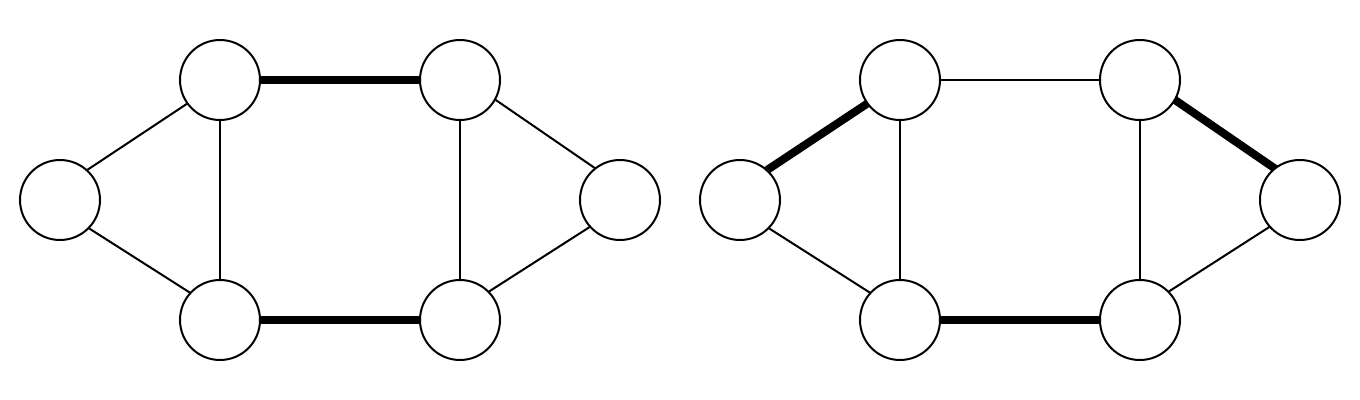
\includegraphics[width=\textwidth]{matchings}
    \caption{A maximal matching and a maximum matching of a graph with 6 vertices. The achieved vertex covers $C$ would have sizes $4$ and $6$ respectively.}
\end{figure}

The maximal matching based algorithm is a 2-approximation to the vertex cover problem. This can be proven by looking at the size of the optimal cover $|C^*|$ and the size of a maximal matching $|M|$. We have $|M| \leq |C^*|$ since every edge in the matching needs to be covered in $C^*$. The size of the vertex cover based on the matching has size $|C| = 2|M|$ and therefore we get that $|C| \leq 2|C^*|$. We can also show that the approximation ratio is tight, by constructing a bipartite graph with equally sized $A$ and $B$ vertex sets, where every element in $A$ is connected to every element in $B$. Here the approximation algorithm will contain all vertices but the minimum vertex cover can be achieved with only the vertices of either $A$ or $B$, which is only half the number of vertices.

\subsection{LP Approximation}
By solving the LP relaxation of the ILP vertex cover formulation and adding every vertex with value at least $1/2$ a vertex cover of at most 2 times the optimal is found. The result is a vertex cover since there exists constraint on each vertex in the following form: $x_i + x_j \ge 1 \text{ for every edge } (i,j) \in E$. Therefore if a variable $x_i$ of vertex $i$ has value below $1/2$ every edge with one endpoint in $i$ must be connected to another vertex with a variable with a value higher than $1/2$ and therefore covered by the approximation algorithm.

To prove that the algorithm is a 2-approximation we define $S^*$ as the optimum vertex cover and $S$ the vertex cover achieved by the algorithm. By summing over the weights of the optimal values of the linear program and using the fact that every $x^*_i \ge 1/2$ for all $i$ in S we can show that $w(S)$ is at most twice of $w(S^*)$ by following equation: $w(S^*) \ge \sum_{i \in S} w_i x^*_i \ge 1/2 \sum_{i \in S} w_i = 1/2 w(S)$.

\newpar Another LP based approximation algorithm is the pricing method. The variables of the dual LP can be seen as prices each edge pays to be part of the cover. The objective of the dual LP is to maximize the profit from edges. The price an edge can pay can be at most the weight of the vertices it is connected to. A vertex $i$ is said to be tight if its dual constraint has no slack, that is we cannot increase the price an edge incident to $i$ without violating the constraints. This creates the base for the pricing approximation algorithm. $Y_e$ is set to 0 for every edge. Then while there exists an edge $(i,j)$ where neither vertex is tight the paid price of edge $e$ is increased until either $i$ or $j$ (or both) becomes tight. The vertex cover is then created from the tight vertices.

\begin{figure}[H]
    \centering
    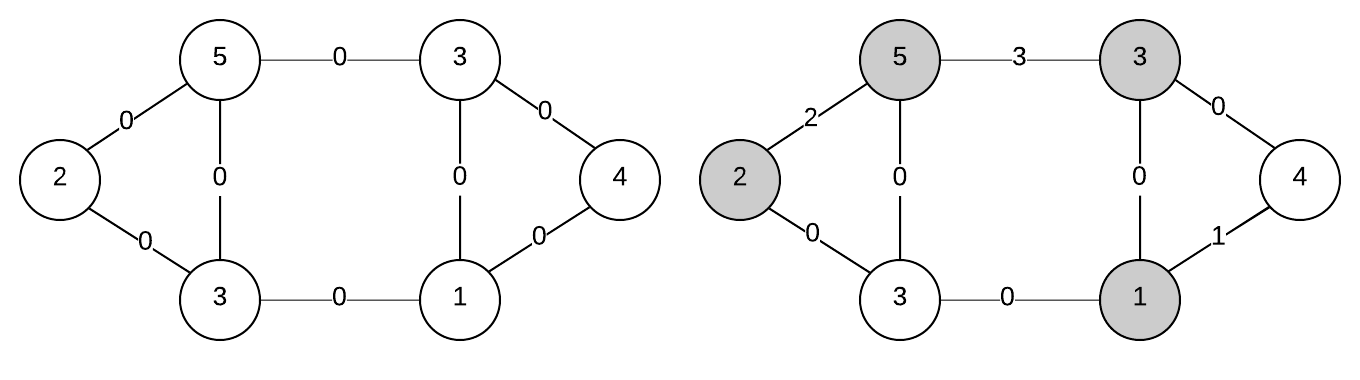
\includegraphics[width=\textwidth]{pricing}
    \caption{The number in each node is the weight of the vertex and the numbers on the edges is the paid price of that edge. The colored vertices are tight.}
\end{figure}

The pricing algorithm is polynomial since at least one vertex is added each iteration of the while loop and the result is a vertex cover since for every edge $(i,j)$ either vertices $i$ or $j$ or both are tight and the edge is therefore covered. 

\newpar Notes on the metric travelling salesman approximation algorithms are left out due to spacial constraints.

\section{Knapsack}
Due to spacial constraints only the $1/\epsilon$-approximation algorithm is explained in these lecture notes. 

In the knapsack problem, $n$ items with a weight and a profit must be packed to optimize profit while adhering to a maximum capacity/volume $V$. This problem is NP-hard but a dynamic programming based pseudo polynomial algorithm exists. Pseudo polynomial means that is it is polynomial in the size of $n$ but the running time is also dependent in the size of the largest possible profit $P$ which can be very large and therefore make the problem very difficult even for small $n$. The approximation algorithm is based on the idea of downscaling $P$ to make the algorithm faster while only creating small errors. The algorithm chooses a scaling factor $K$ based on the wanted ratio to optimality $K=\epsilon P/n$, then for each object $p^*_i = \lfloor p_i/K \rfloor$.

For example if we have the following profits $\{ 150, 100, 95, 5 \}$ and we assume $P=200$. If we want a 1/2-approximation scheme we find $K=\frac{1/2*200}{4} = 25$. The profits are then scaled to $\{ 6, 4, 3, 0 \}$. Note here that we floor $95/25=3.8$ and $5/25=0.2$ which means we loose some precision from the original problem. The two other profits keep their ratio.

\newpar The running time is $\mathcal{O}(n^2 \lfloor P/K \rfloor) \equiv \mathcal{O}(n^2 \lfloor n/\epsilon \rfloor)$ and is therefore an example of an algorithm which is both polynomial in $n$ and in $1/\epsilon$ and hence is a FPTAS. We can furthermore see that the solution obtained is at most $1+\epsilon$ from optimal by the following proof. Let $O$ be the optimal solution, $S$ be the solution from the approximation algorithm, $p(x)$ be the profit of the solution $x$ given the unscaled profits and $p^*(x)$ given the scaled profits. Since there are $n$ objects and the profit of each object is at most scaled by K we get $p(O) - K p^*(O) \le n K$. Then we have $p(S) \ge K p^*(O) \ge p(O)-n K$. By using the definition of $K$ $n K$ becomes $n (\epsilon P/n)$ and we get $p(S) \ge p(O) - \epsilon P \ge (1-\epsilon) p(O)$. This shows us that the scaling algorithm is a $(1+\epsilon)$-approximation algorithm to the knapsack problem.
